% !TeX root = ../documento.tex
\chapter{O Estado da Arte}
\label{cap:o-estado-da-arte}

Este capítulo apresenta uma análise histórica e técnica do componente alvo desta pesquisa, o sistema de freio. São explorados os principais marcos e inovações tecnológicas, bem como os diferentes tipos de freios e sua evolução mecânica e elétrica. São descritos os componentes e seus princípios de funcionamento, além de serem discutidos estudos experimentais e teóricos, desafios, limitações e tendências de aplicação. O objetivo é fornecer subsídios para a compreensão do contexto atual e identificar oportunidades para futuras contribuições acadêmicas.


\section{Histórico dos Sistemas de Freio}
\label{sec:o-estado-da-arte-1}


\subsection{Evolução dos Sistemas de Freio ao Longo do Tempo}
\label{sec:o-estado-da-arte-1-1}
Os sistemas de freio passaram por diversas etapas de desenvolvimento, desde métodos rudimentares utilizados em carruagens na antiguidade até sistemas eletrônicos modernos e freios regenerativos. A literatura destaca que essas transformações ocorreram de forma gradual, acompanhando avanços tecnológicos e demandas de segurança veicular.


\subsection{Principais Marcos e Inovações Tecnológicas}
\label{sec:o-estado-da-arte-1-2}
Inicialmente, os freios eram simples, como o uso de varas de madeira contra as rodas. Em 1850, foi introduzido o freio de sapata em carruagens REIF (2014). No século XVIII, o uso de freios de fricção entre um rotor e um estator foi introduzido em carruagens puxadas por cavalos e, posteriormente, adaptado para veículos automotivos no final do século XIX BRYANT (2022). A patente do freio a disco ocorreu em 1902 por George Westinghouse, embora sua adoção em massa tenha ocorrido apenas na década de 1950 \cite{Konrad2014}.

A introdução do sistema hidráulico na década de 1920, pelo engenheiro americano Tom Reilly, permitiu uma distribuição mais uniforme da força de frenagem \cite{Lentin2022}, substituindo sistemas mecânicos (como cabos ou varas) por fluido. Os freios de tambor nas quatro rodas se popularizaram nesse período, evoluindo para freios a disco a partir de 1959 \cite{Konrad2014}. O desenvolvimento do \textit{Anti-lock Braking System} (ABS) na década de 1970, que revolucionou a segurança veicular, representou um avanço importante ao permitir o controle direcional durante a frenagem \cite{AndrewJ2022}.

A transição para sistemas de freio \textit{"by-wire"} (sem conexão mecânica direta) é destacada como um marco relevante a partir dos anos 1990 \cite{Donghai2022}. Entre os avanços recentes, destacam-se sistemas eletrônicos como Controle Eletrônico de Estabilidade (ESC), Distribuição Eletrônica de Frenagem (EBD), Sistema de Frenagem Autônoma de Emergência (AEB) \cite{Lentin2022}, sistemas de freio adaptativos e frenagem regenerativa.

Em suma, os sistemas de frenagem veicular têm experienciado um avanço tecnológico substancialmente acelerado, especialmente nas últimas décadas, superando o progresso acumulado ao longo de séculos anteriores.

Isso porque, enquanto os séculos XIX e XX foram marcados por evoluções mecânicas e hidráulicas lentas e graduais, o século XXI, promovido especialmente por inovações em eletrônica, inteligência artificial e interoperabilidade de sistemas, promoveu uma revolução qualitativa nos mecanismos de frenagem. A Figura~\ref{fig:trajetoria_historica_evolucao_tecnologia_adas} apresenta esta evolução em níveis.

Essa transformação se reverbera não apenas no avanço técnico, mas também em uma mudança de paradigma na função do sistema de frenagem, que passa a atuar como elemento ativo na prevenção de acidentes, melhora da segurança, além de contribuir para a conveniência e conforto na direção, conforme é demonstrado na Figura~\ref{fig:trajetoria_historica_evolucao_tecnologia_adas}.

\begin{figure}[htbp]
    \centering
    \caption{Trajetória da automação dos veículos nas últimas décadas.}
    \label{fig:trajetoria_historica_evolucao_tecnologia_adas}
    \fbox{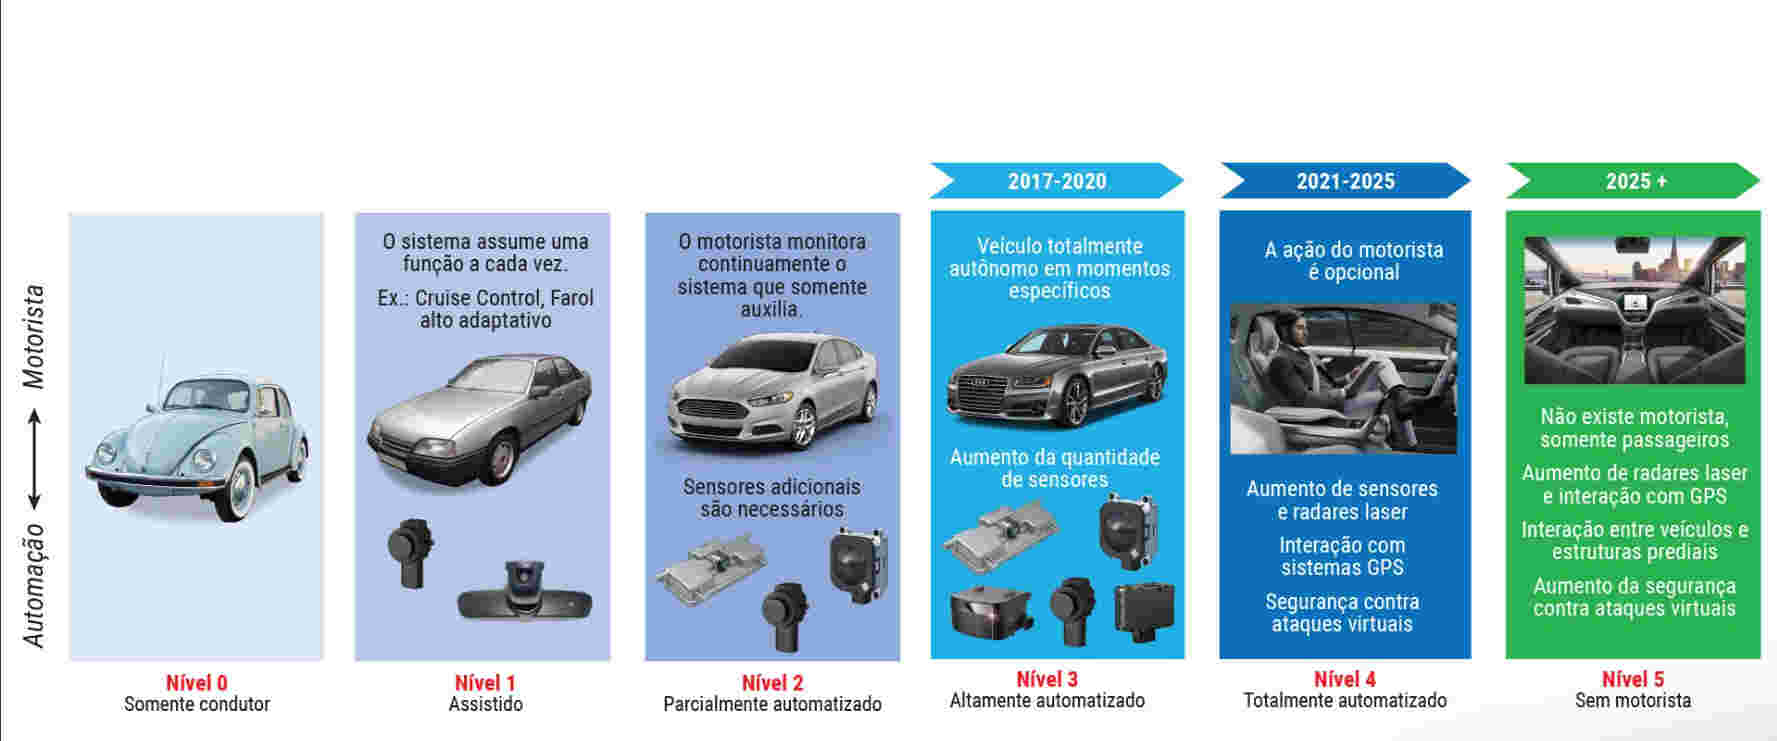
\includegraphics[width=0.8\textwidth]{figuras/trajetoria_historica_evolucao_tecnologia_adas.jpg}}
    \fonte{ O Autor, adaptado de \cite{evolucaodosistemaemniveis2022}. }
\end{figure}

\section{Classificação dos Sistemas de Freio}
\label{sec:o-estado-da-arte-1-3}
Os sistemas de freio podem ser classificados em várias categorias, segundo o princípio de funcionamento e aplicação. Conforme discutido por \citeonline{Konrad2014} e \citeonline{Lentin2022}, existem sistemas que geram atrito para reduzir a velocidade do veículo, como o freio a tambor, que utiliza sapatas que se expandem contra um tambor para gerar atrito, e o freio a disco, que utiliza pastilhas pressionando um disco rotativo \cite{Lentin2022}.

%Sistemas híbridos, que combinam freios a disco nas rodas dianteiras e freios a tambor nas rodas traseiras \cite{Lentin2022}, ainda são comuns em veículos econômicos devido ao custo-benefício. Essa configuração é frequentemente adotada por fabricantes para equilibrar eficiência, custo de produção e manutenção, além de considerar a distribuição de peso do veículo, já que a maioria do peso está na dianteira, onde os freios a disco são mais eficientes, enquanto os freios a tambor são adequados para a traseira, onde a frenagem é menos intensa.

Sistemas híbridos, que combinam freios a disco nas rodas dianteiras e freios a tambor nas rodas traseiras \cite{Lentin2022}, ainda são comuns em veículos econômicos devido ao custo-benefício. Essa configuração é frequentemente adotada por fabricantes por equilibrar desempenho e custo, uma vez que, durante a frenagem, ocorre a transferência dinâmica de carga para o eixo dianteiro, que demanda maior capacidade de dissipação térmica — característica típica dos freios a disco — enquanto o eixo traseiro está sujeito a menores esforços, sendo adequadamente atendido por freios a tambor \cite{Rudolf2011}.

Os sistemas de freio regenerativos, utilizados em veículos híbridos e elétricos, permitem a recuperação de energia durante a frenagem. Nesses sistemas, a energia gerada durante a frenagem é convertida em eletricidade e armazenada na bateria do veículo, promovendo maior eficiência energética e autonomia \cite{Donghai2022}. Estudos recentes publicados em periódicos como IEEE \textit{Transactions on Vehicular Technology} destacam o potencial desses sistemas para contribuir com a sustentabilidade e eficiência dos veículos elétricos, embora ressaltem desafios relacionados à integração com sistemas convencionais de frenagem e à validação em diferentes condições de operação \cite{Kumar2024}.

Além disso, alternativas modernas incluem sistemas eletro-hidráulicos, que utilizam controle eletrônico para regular a pressão hidráulica aplicada às pinças de freio, e sistemas eletromagnéticos, que interagem diretamente com o sistema de movimento do veículo, especialmente em aplicações de veículos autônomos \cite{Donghai2022}.

Ainda relacionado aos sistemas eletro-hidráulicos, estudos recentes também demonstram a relevância do projeto paramétrico de motores integrados a sistemas de freio eletro-hidráulicos em veículos elétricos, evidenciando ganhos em eficiência e resposta dinâmica \cite{MotorParametricDesign2023}. Adicionalmente, estratégias de controle coordenado de pressão têm sido propostas para aprimorar a precisão e robustez desses sistemas, conforme discutido em \citeonline{PressureCoordinatedControl2023}. A literatura técnica explora a potencial aplicação dessas alternativas, destacando a necessidade de análises experimentais e validações em ambientes reais para avaliar sua eficiência e confiabilidade.

Portanto, a classificação dos sistemas de freio apresentada neste capítulo busca contribuir para a compreensão das diferentes tecnologias disponíveis e, possíveis soluções que podem ser exploradas em contextos acadêmicos e industriais. A análise das configurações e princípios de funcionamento dos sistemas de freio é fundamental para validar modelos matemáticos e estratégias de controle, bem como para identificar limitações e oportunidades de investigação na área de sistemas automotivos.


\section{Tipos de Sistemas de Freio}
\label{sec:o-estado-da-arte-2}


\subsection{Freios a disco e a tambor}
\label{sec:o-estado-da-arte-2-1}
Os freios a disco e a tambor são os dois principais tipos de sistemas de freio utilizados em veículos. Os freios a disco (Figura~\ref{fig:freio-disco}) são conhecidos por sua eficiência na dissipação de calor, durabilidade e desempenho consistente em diferentes condições de operação. São amplamente utilizados em veículos modernos, especialmente nas rodas dianteiras e, cada vez mais, nas traseiras \cite{Konrad2014}. Eles utilizam pastilhas que são pressionadas contra um disco rotativo, proporcionando desempenho de frenagem adequado em altas velocidades \cite{AndrewJ2022}.

\begin{figure}[htbp]
    \centering
    \caption{Freio a Disco.}
    \label{fig:freio-disco}
    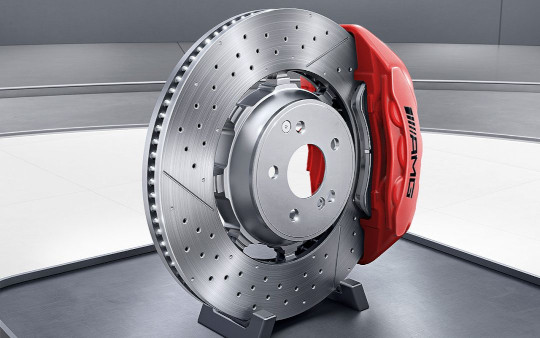
\includegraphics[width=0.8\textwidth]{figuras/freio-disco.jpg}
    \fonte{ O Autor, adaptado de \cite{freioadisco2023}. }
\end{figure}

A literatura técnica apresenta diversas análises sobre o desempenho térmico e desgaste dos freios a disco, destacando sua potencial aplicação em veículos de passeio e comerciais \cite{Reboucas2025}. Estudos experimentais e simulações computacionais têm contribuído para a validação de modelos matemáticos que descrevem o comportamento desses sistemas sob diferentes condições de carga e temperatura \cite{ChenQuguang2019}. Tais contribuições oferecem subsídios para futuras pesquisas voltadas à otimização de materiais de fricção e ao desenvolvimento de estratégias de controle para sistemas de freio.

Por outro lado, os freios a tambor (Figura~\ref{fig:freio-tambor}) utilizam sapatas com revestimento de material de fricção (abrasivo), que se expandem contra a superfície interna de um tambor. Estes sistemas são mais econômicos e ainda comuns em veículos menores e de baixo custo \cite{Konrad2014}. A análise de sua eficiência e durabilidade é tema recorrente em estudos acadêmicos, que também exploram suas limitações, especialmente relacionadas à dissipação de calor e ao desgaste dos componentes \cite{Reboucas2025}.

\begin{figure}[htbp]
    \centering
    \caption{Freio a Tambor.}
    \label{fig:freio-tambor}
    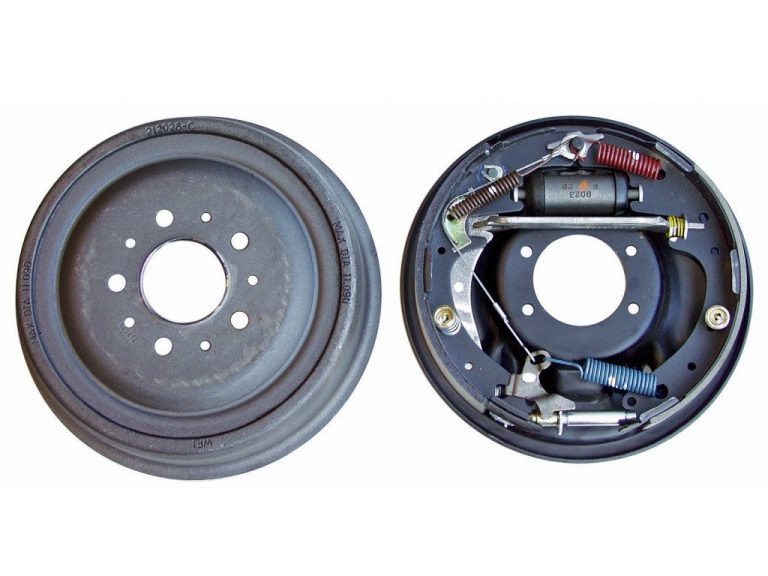
\includegraphics[width=0.8\textwidth]{figuras/freio-tambor.jpg}
    \fonte{ O Autor, adaptado de \cite{freioATambor}. }
\end{figure}

A escolha entre freios a disco e a tambor depende de fatores como custo, distribuição de peso do veículo, intensidade da frenagem exigida e requisitos de manutenção. A literatura sugere que sistemas híbridos, combinando ambos os tipos, podem ser uma alternativa viável para determinadas aplicações, especialmente em veículos econômicos \cite{AmbeMohammedHussein2024}.

Essas análises e explorações favorecem o entendimento das potencialidades e limitações dos sistemas de freio, oferecendo contribuições para a validação de modelos e desenvolvimento de novas soluções na área automotiva.


\subsection{Sistemas de Freio Hidráulico e Pneumático}
\label{sec:o-estado-da-arte-2-2}
Os sistemas de freio podem ser classificados em hidráulicos e pneumáticos. Os sistemas hidráulicos. Figura~\ref{fig:sistemas_hidraulicos}, que utilizam fluido de freio para transmitir a força do pedal aos freios, são os mais comuns em veículos leves \cite{Konrad2014, AndrewJ2022}. Esses sistemas incluem componentes como cilindros mestres, válvulas de controle de pressão e sistemas de reforço (\textit{boosters}) \cite{Rudolf2011}.

\begin{figure}[htbp]
    \centering
    \caption{Sistemas Hidráulicos.}
    \label{fig:sistemas_hidraulicos}
    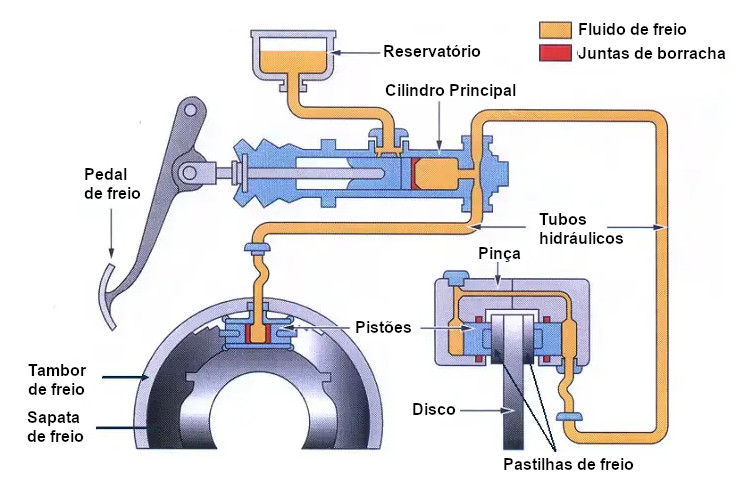
\includegraphics[width=0.8\textwidth]{figuras/sistemas_hidraulicos.jpg}
    \fonte{ O Autor, adaptado de \cite{sistemahidraulico}. }
\end{figure}

Já os sistemas pneumáticos. Figura~\ref{fig:sistemas_pneumatico}, que utilizam ar comprimido ou outro gás pressurizado para aplicar a força de frenagem, são predominantes em veículos pesados, como caminhões e ônibus \cite{Konrad2014}. De acordo com análises recentes, esses sistemas apresentam potencial aplicação em veículos de grande porte devido à sua capacidade de gerar força suficiente para frear veículos com grande massa, além de serem reconhecidos por sua durabilidade e segurança operacional \cite{BuHanShue2007}.

\begin{figure}[htbp]
    \centering
    \caption{Sistemas Pneumáticos.}
    \label{fig:sistemas_pneumatico}
    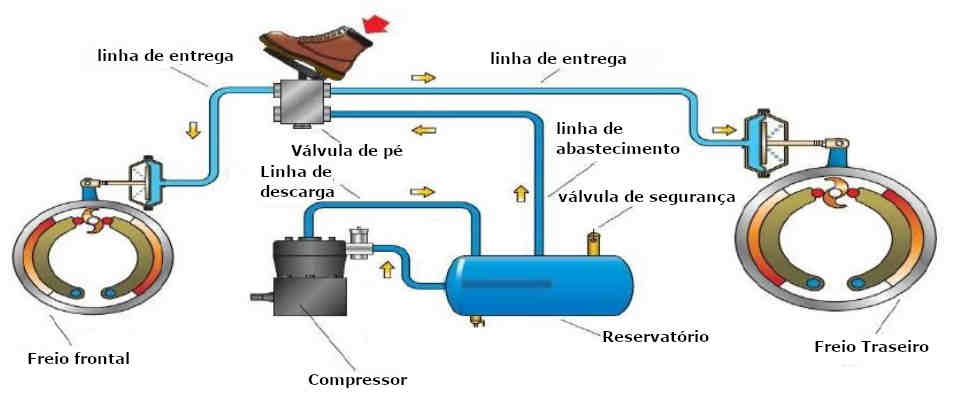
\includegraphics[width=0.8\textwidth]{figuras/sistemas_pneumatico.jpg}
    \fonte{ O Autor, adaptado de \cite{sistemapneumaticos}. }
\end{figure}

\subsection{Tecnologias Modernas}
\label{sec:o-estado-da-arte-2-3}
As tecnologias modernas têm contribuído para avanços na segurança, eficiência e desempenho dos veículos \cite{Konrad2014}. A capacidade dos sistemas de freio de fornecer desaceleração controlada e estável, mesmo em condições adversas, tem sido examinado e corroborado por inúmeras investigações acadêmicas \cite{AndrewJ2022}.

O ABS (\textit{Anti-lock Braking System}), por exemplo, evita o travamento das rodas durante a frenagem \cite{Donghai2022}, sendo considerada uma das tecnologias mais amplamente utilizadas em veículos modernos. Estudos recentes exploram o potencial do ABS para melhorar o controle do veículo e reduzir o risco de derrapagem, especialmente em pisos escorregadios \cite{Rajkumar2024}. A modulação da pressão de frenagem permite que o motorista mantenha o controle do veículo durante frenagens de emergência, sendo uma contribuição relevante para a segurança veicular \cite{Rajkumar2024}.

O ABS possui papel indispensável na segurança ao preservar a dirigibilidade e o controle direcional do veículo durante frenagens intensas, reduzindo o risco de derrapagem por travamento. Em algumas condições de baixa aderência e/ou superfícies soltas, a distância de frenagem pode não ser minimizada em relação ao bloqueio total, mas o benefício principal do ABS permanece associado à estabilidade e capacidade de manobra \cite{Rudolf2011, Lentin2022}.

Além do uso clássico em frenagem comandada pelo condutor, a mesma infraestrutura eletro-hidráulica de unidades ABS/ESC é empregada por funções como ESC e aplicações ADAS (por exemplo, ACC/AEB) para realizar intervenções de \textbf{frenagem ativa}, impondo perfis de pressão por roda a partir de referências geradas eletronicamente.
Além do ABS, outras tecnologias complementares têm sido amplamente exploradas e validadas, tais como:

\begin{itemize}
    \item \textbf{ESC (Controle Eletrônico de Estabilidade):} O ESC corrige a trajetória do veículo em situações de derrapagem como indicado na Figura~\ref{fig:controle_eletronico_estabilidade}, integrando-se ao ABS para fornecer um controle preciso da força de frenagem \cite{Konrad2014, Lentin2022}. Estudos destacam o potencial do ESC para contribuir com a estabilidade veicular em situações críticas \cite{Donghai2022}.

          \begin{figure}[htbp]
              \centering
              \caption{Controle Eletrônico de Estabilidade (ESC).}
              \label{fig:controle_eletronico_estabilidade}
              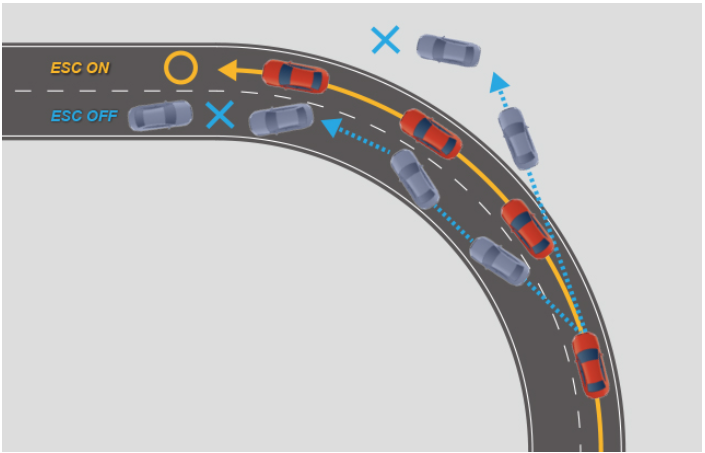
\includegraphics[width=0.8\textwidth]{figuras/controle_eletronico_estabilidade.jpg}
              \fonte{ O Autor, adaptado de \cite{controleeletronicodeestabilidadeESC}. }
          \end{figure}

    \item \textbf{EBD (Distribuição Eletrônica de Frenagem):} O EBD distribui a força de frenagem de forma equilibrada entre os eixos, melhorando a estabilidade do veículo \cite{Konrad2014}. Esse sistema é especialmente útil em veículos com carga variável, garantindo uma frenagem eficiente em todas as condições \cite{Rudolf2011}.

    \item \textbf{BAS (Assistência de Frenagem):} O BAS aumenta a pressão de frenagem durante emergências, mesmo que o motorista não aplique força suficiente no pedal, garantindo uma frenagem eficaz e segura \cite{Donghai2022}.

    \item \textbf{TCS (Sistema de Controle de Tração):} O TCS evita a derrapagem das rodas motrizes ao reduzir o torque do motor ou aplicar os freios, melhorando a tração e a estabilidade do veículo em superfícies escorregadias \cite{Donghai2022}, Figura~\ref{fig:sistema_controle_tracao}. Em outras palavras, controla o deslizamento das rodas durante a aceleração \cite{Konrad2014, Lentin2022}.

          \begin{figure}[htbp]
              \centering
              \caption{Demostração da roda sem (TCS).}
              \label{fig:sistema_controle_tracao}
              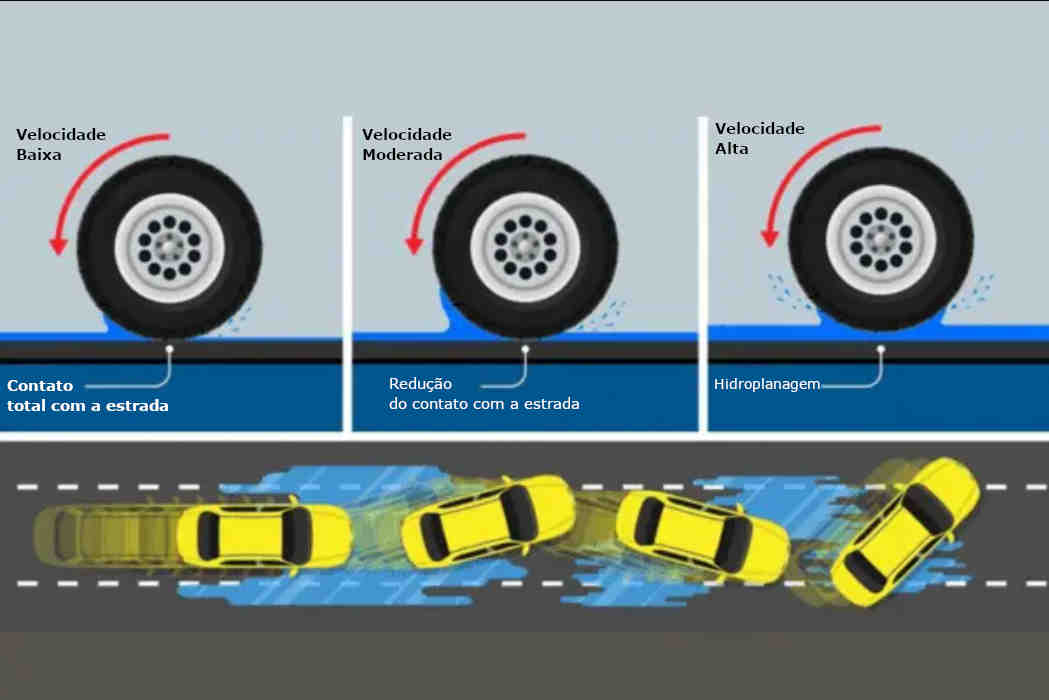
\includegraphics[width=0.8\textwidth]{figuras/sistema_controle_tracao.jpg}
              \fonte{ O Autor, adaptado de \cite{demostracaodarodasemTCS}. }
          \end{figure}

    \item \textbf{ACC (Controle de Cruzeiro Adaptativo):}  ajusta automaticamente a velocidade do veículo com base no tráfego à frente, mantendo uma distância segura em relação ao veículo precedente \cite{Konrad2014, Rudolf2011, Lentin2022}. Para isso, o sistema utiliza predominantemente sensores de radar instalados na parte frontal do veículo, capazes de medir continuamente a distância e a velocidade relativa dos veículos à frente, permitindo a adaptação dinâmica da velocidade de cruzeiro, conforme ilustrado na Figura~\ref{fig:acc-controle-de-cruzeiro-adaptativo}.

          \begin{figure}[htbp]
              \centering
              \caption{Controle de Cruzeiro Adaptativo (ACC).}
              \label{fig:acc-controle-de-cruzeiro-adaptativo}
              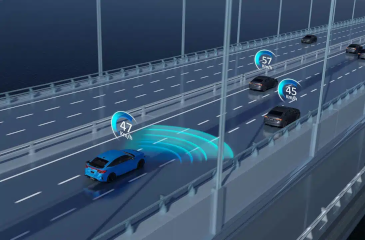
\includegraphics[width=0.8\textwidth]{figuras/acc-controle-de-cruzeiro-adaptativo.png}
              \fonte{ O Autor, adaptado de \cite{acc-controle-cruzeiro-adaptativo}. }
          \end{figure}

          Tendo em vista esses diferentes sistemas, o ADAS (Sistemas Avançados de Assistência ao Motorista) constitui um conjunto de tecnologias de assistência que pode integrar diversos desses recursos e empregar sensores, câmeras e outros dispositivos eletrônicos a fim de aumentar a segurança veicular e melhorar a experiência de condução. \cite{Konrad2014}


\end{itemize}

\section{Componentes dos Sistemas de Freio}
\label{sec:o-estado-da-arte-2-4}
Os sistemas de freio automotivo são compostos por diversos elementos, cuja configuração depende do tipo de tecnologia empregada. Nos sistemas de freio a disco e a tambor, destacam-se discos, tambores, pastilhas, sapatas e lonas, cada um desempenhando funções específicas na geração do atrito necessário para desacelerar o veículo. Sistemas hidráulicos incorporam cilindros mestres, válvulas de controle de pressão e servofreios, enquanto sistemas pneumáticos utilizam compressores de ar, válvulas e câmaras de freio \cite{Rudolf2011, Konrad2014, Lentin2022, AndrewJ2022}.

A presença de sensores, como os de velocidade das rodas, pressão e temperatura, é fundamental para o funcionamento de sistemas eletrônicos de frenagem, como ABS, ESC e ADAS. Esses sensores monitoram parâmetros críticos e permitem a atuação precisa dos sistemas de controle, contribuindo para a análise do desempenho em diferentes condições operacionais \cite{Konrad2014, Lentin2022}. Atuadores eletrônicos, como motores elétricos e mecanismos piezoelétricos, têm sido explorados em aplicações de freio \textit{“by-wire”} e freio eletrônico de estacionamento (EPB), ampliando as possibilidades de integração com sistemas avançados de assistência ao motorista \cite{HouhuaJingShihao2023}.

Além dos componentes tradicionais, a literatura discute o uso de materiais alternativos, como discos de cerâmica e carbono, que apresentam potencial para melhorar a dissipação de calor e a resistência ao desgaste, embora seu emprego ainda seja restrito por questões de custo e disponibilidade \cite{Lentin2022}. A escolha dos materiais de fricção, bem como o desenvolvimento de sensores e atuadores mais eficientes, permanece como tema de investigação, oferecendo oportunidades para reconhecimento de novos modelos e estratégias de controle.

\subsection{Descrição, Função e Importância dos principais componentes }
\label{sec:o-estado-da-arte-3-1}
Os principais componentes dos sistemas de freio desempenham funções essenciais para a segurança e eficiência do veículo:

\begin{itemize}
    \item \textbf{Discos e tambores:} Os discos de freio, geralmente feitos de ferro fundido ou aço, possuem variações ventiladas para melhor dissipação de calor \cite{Konrad2014}. Já os tambores de freio são compostos por sapatas e lonas que pressionam a superfície interna do tambor para gerar atrito \cite{Konrad2014}.
          Discos de cerâmica também são utilizados devido à sua capacidade de dissipação rápida de calor \cite{Lentin2022}.

          São responsáveis por dissipar a energia cinética do veículo, transformando-a em calor. A eficiência térmica e a resistência ao desgaste são fundamentais para garantir a segurança e a durabilidade do sistema de freio \cite{Rudolf2011, AndrewJ2022}.

    \item \textbf{Pastilhas e lonas:} As pastilhas de freio são feitas de materiais que oferecem alta resistência ao desgaste e ao calor, aplicando pressão nos discos para gerar atrito \cite{Konrad2014, Lentin2022}. As lonas de freio, utilizadas em sistemas de freio a tambor, possuem composições semelhantes às pastilhas e aplicam pressão nos tambores para gerar atrito \cite{Konrad2014, Lentin2022}.
          De modo que, a partir desse atrito, geram a força de frenagem necessária para parar o veículo. A escolha de materiais de fricção adequados é essencial para garantir alta resistência ao desgaste e ao calor \cite{Konrad2014, AndrewJ2022}.

    \item \textbf{Cilindros mestres e servofreios:} O cilindro mestre converte a força do pedal em pressão na linha hidráulica, distribuindo-a para os freios \cite{Konrad2014, Lentin2022}. O servofreio amplifica a força aplicada pelo motorista, utilizando vácuo do motor ou pressão hidráulica \cite{Konrad2014}. Garantindo que a força aplicada no pedal seja transmitida de forma eficiente para os freios, convertendo a força mecânica em pressão na linha do sistema hidráulico \cite{Konrad2014,Lentin2022}.

    \item \textbf{Sensores:} Sensores de velocidade das rodas são essenciais para sistemas como ABS e TCS, monitorando exclusivamente a velocidade das rodas \cite{Konrad2014, Lentin2022, AndrewJ2022}. Já a pressão do fluido de freio é monitorada por sensores de pressão específicos instalados no circuito hidráulico. Sensores de temperatura também auxiliam na análise do desempenho do sistema \cite{Konrad2014}. Esses sinais asseguram o funcionamento correto dos sistemas eletrônicos de frenagem, como ABS e ESC \cite{Konrad2014, AndrewJ2022}.

\end{itemize}


\subsection{Princípios de Funcionamento}
\label{sec:o-estado-da-arte-3-3}
Em suma, os sistemas de freio funcionam com base em princípios hidráulicos e mecânicos. Quando o pedal de freio é pressionado, a força aplicada pelo motorista é transmitida à haste do pedal e, em seguida, ao servofreio (quando presente), que amplifica essa força. Na sequência, o cilindro mestre converte essa força amplificada em pressão na linha hidráulica, que é então distribuída para os freios nas rodas por meio do circuito hidráulico \cite{Konrad2014, Lentin2022, Konrad2014}. Nos freios a disco, as pastilhas pressionam os discos, gerando atrito e dissipando energia cinética em forma de calor. Nos freios a tambor, as lonas pressionam a superfície interna dos tambores para gerar atrito de maneira similar \cite{Konrad2014, Lentin2022}.

Por outro lado, os sensores de velocidade das rodas monitoram continuamente as condições de rotação das rodas, mas não ajustam a pressão. A interpretação desses sinais é realizada pela unidade de controle eletrônico, que então \textbf{modula a pressão e a força de frenagem} por meio das válvulas e da bomba do sistema, assegurando a atuação correta de sistemas como ABS e ESC \cite{Konrad2014, AndrewJ2022}.

\begin{comment}
Em suma, os sistemas de freio funcionam com base em princípios hidráulicos e mecânicos. Quando o pedal de freio é pressionado, o cilindro mestre converte essa força em pressão hidráulica, distribuída para os freios nas rodas. Nos freios a disco, as pastilhas pressionam os discos, gerando atrito e dissipando a energia cinética em forma de calor. Nos freios a tambor, as lonas pressionam a superfície interna dos tambores, gerando atrito de maneira similar \cite{Konrad2014, Lentin2022}.

Por outro lado, os sensores de velocidade das rodas monitoram continuamente o desempenho do sistema de freio, ajustando  a pressão e a força de frenagem conforme necessário para garantir a segurança e a eficiência do veículo \cite{Konrad2014, AndrewJ2022}.

% esta subsecao foi comentado por motivo de orientacao na revisao pela banca

\section{Mecanismos de ação dos diferentes tipos de freio}
\label{sec:o-estado-da-arte-4}
Os sistemas de freio são essenciais para a segurança dos veículos, convertendo energia cinética em calor através do atrito. Existem diferentes tipos de freios, cada um com seus mecanismos específicos de ação.

\begin{itemize}
    \item \textbf{Freios a Tambor:} Nos freios a tambor, as lonas são pressionadas contra a superfície interna do tambor, também gerando atrito \cite{Konrad2014, Lentin2022}. Embora menos eficientes que os freios a disco, são comuns em veículos mais antigos e em sistemas de freio de estacionamento \cite{AndrewJ2022}.


    \item \textbf{Freios a Disco:} Os freios a disco funcionam pela pressão hidráulica que move as pastilhas contra o disco, gerando atrito e desacelerando o veículo \cite{Konrad2014, Lentin2022}. Esse sistema é eficiente e oferece uma resposta rápida, sendo amplamente utilizado em veículos modernos \cite{Rudolf2011}.



    \item \textbf{Sistemas Eletro-Hidráulicos e Eletromagnéticos:} Os sistemas eletro-hidráulicos e eletromagnéticos utilizam a geração de torque de frenagem e a regulação de pressão para distribuir a força entre os eixos dianteiro e traseiro, garantindo uma frenagem equilibrada \cite{Donghai2022}.
\end{itemize}
\end{comment}

%################################################################
%################################################################
%################################################################
\section{Revisão de estudos experimentais e teóricos sobre a eficiência e desempenho dos sistemas de freio}
\label{sec:o-estado-da-arte-5}
Diversos estudos destacam a relevância dos sistemas de freio para a segurança veicular. Pesquisas indicam que a integração de tecnologias como ABS e ESC está associada à redução do risco de acidentes, especialmente em condições adversas \cite{Rudolf2011, Donghai2022}. O desenvolvimento de sistemas de freio mais eficientes e a implementação de novas tecnologias continuam sendo temas de interesse para a indústria automotiva \cite{AndrewJ2022}.

Entre as abordagens experimentais, são realizados testes de frenagem em diferentes superfícies, como seca, molhada e com gelo, além da análise do desgaste de componentes \cite{Konrad2014}. Estudos sobre materiais de atrito, como pastilhas e discos, buscam compreender fatores que influenciam a durabilidade e eficiência dos freios \cite{Lentin2022}. Outros trabalhos discutem a distribuição da força de frenagem e o controle de modos de frenagem, incluindo a comparação entre frenagem regenerativa e por atrito, especialmente em sistemas híbridos \cite{Donghai2022}.

Além disso, investigações sobre o impacto dos materiais de atrito no desempenho dos freios consideram aspectos como temperatura, desgaste e distribuição de pressão \cite{Rudolf2011}. Estudos recentes também destacam a importância de modelar a evolução do coeficiente de atrito das lonas de freio para aprimorar a estimação da pressão de frenagem, especialmente em situações onde a medição direta é limitada ou sujeita a incertezas \cite{ZhangWang2021}.

Adicionalmente, pesquisas sobre o projeto paramétrico de motores em sistemas de freio eletro-hidráulicos têm demonstrado avanços na integração entre controle eletrônico e desempenho dinâmico, especialmente em veículos elétricos \cite{MotorParametricDesign2023}. A geração de \gls{NVH} também é objeto de análise, com estudos avaliando o comportamento de diferentes compostos de fricção sob variadas condições de operação \cite{AndrewJ2022}.

Cabe mencionar que pesquisas recentes têm explorado a influência da eletrônica embarcada e dos sensores inteligentes na avaliação do desempenho dos sistemas de freio \cite{Lentin2022}, especialmente em aplicações que envolvem ADAS e condução autônoma. A validação experimental e computacional desses sistemas contribui para o entendimento das limitações e potencialidades das tecnologias atuais, oferecendo subsídios para futuras investigações e desenvolvimento de soluções mais seguras e eficientes.

%################################################################
%################################################################
%################################################################
\section{Análise de dados de testes em simulações de frenagem}
\label{sec:o-estado-da-arte-5-1}
A avaliação do desempenho dos sistemas de freio é realizada por meio de diferentes métodos experimentais e computacionais. Testes práticos em pistas de prova, como os realizados no centro de testes da Bosch em \textit{Boxberg} Alemanha, permitem observar o comportamento dos sistemas em situações reais, incluindo frenagens de emergência, descidas prolongadas e fadiga térmica \cite{Rudolf2011}. Tais experimentos possibilitam a análise da resposta dos sistemas ABS e ESC/ESP (\textit{Electronic Stability Control}/\textit{Electronic Stability Program}), que atuam de forma integrada para promover maior estabilidade e segurança.

Além dos ensaios em campo, simulações computacionais têm sido amplamente utilizadas para prever o desempenho dos freios sob variadas condições de uso \cite{Lentin2022}. Modelos matemáticos e simulações em dinamômetros auxiliam na compreensão dos efeitos da temperatura, velocidade e tipo de material de fricção sobre a eficiência de frenagem \cite{AndrewJ2022}.

A utilização de bancadas de teste, como HIL \textit{hardware-in-the-loop}, contribuem para a validação de sistemas híbridos e regenerativos, permitindo a exploração de diferentes cenários operacionais \cite{Donghai2022}. Estudos como o de \cite{Lv2014} demonstram a eficácia da simulação HIL para testar estratégias de modulação de pressão em sistemas de freio hidráulico integrados à frenagem regenerativa em veículos elétricos.

A análise dos dados obtidos em testes e simulações fornece subsídios para o desenvolvimento de estratégias de controle e identificação de limitações dos sistemas atuais. Diversas pesquisas têm explorado a influência de variáveis ambientais, como umidade e temperatura, na resposta dos sistemas de freio, destacando a importância da validação em condições reais de operação. A integração de sensores avançados e algoritmos inteligentes representa uma potencial aplicação para aprimorar o monitoramento e a atuação dos sistemas de frenagem, especialmente em veículos equipados com ADAS\cite{KapinskiJamesDeshmukh2016}.

%################################################################
%################################################################
%################################################################
\section{Desafios e Limitações dos Sistemas de Freio Modernos}
\label{sec:o-estado-da-arte-5-2}
A pesquisa e o desenvolvimento de sistemas de freio automotivos enfrentam diversos desafios técnicos e tecnológicos. Entre as principais dificuldades, destaca-se a necessidade de materiais de atrito que conciliem eficiência, durabilidade e custo acessível, considerando o contexto competitivo do setor \cite{AndrewJ2022}. O desempenho dos freios sob diferentes condições de uso demanda simulações avançadas e testes extensivos, que buscam validar modelos matemáticos e prever o comportamento dos sistemas em situações reais \cite{Lentin2022}.

A integração de sistemas de freio com tecnologias autônomas e híbridas apresenta obstáculos relacionados à precisão dos sensores e atuadores, bem como à interoperabilidade entre diferentes módulos eletrônicos \cite{Donghai2022, Lentin2022}. Questões como a dependência de sensores em ambientes adversos, a eficiência energética dos sistemas eletromagnéticos e a necessidade de materiais de fricção mais leves e resistentes continuam sendo objeto de análise e discussão na literatura técnica.

Além disso, o gerenciamento térmico e a dissipação de energia durante frenagens intensas representam áreas que demandam aprimoramentos contínuos. O desenvolvimento de estratégias para minimizar o desgaste irregular de componentes e a influência de variáveis ambientais, como umidade e temperatura, permanece como tema relevante para futuras investigações \cite{Konrad2014, Rudolf2011}.

Outro aspecto que merece atenção é a segurança cibernética dos sistemas de freio conectados, especialmente em veículos equipados com ADAS e funções autônomas. A proteção contra ataques e falhas de comunicação é fundamental para garantir a confiabilidade dos sistemas em cenários de mobilidade inteligente.

Em síntese, os desafios enfrentados pelos sistemas de freio modernos refletem a complexidade crescente das demandas automotivas, exigindo abordagens multidisciplinares e validações rigorosas. A análise crítica dessas limitações contribui para orientar pesquisas futuras e o desenvolvimento de soluções mais robustas e seguras para o setor.

\section{Síntese crítica e posicionamento do trabalho}
\label{sec:estado-arte-sintese-critica}

Apesar de o sistema de freio aparecer, na literatura, ora como componente mecânico-hidráulico (com foco em materiais, eficiência térmica e durabilidade) ora como parte de arquiteturas eletrônicas (ABS/ESC/ADAS), o recorte deste trabalho exige uma leitura mais específica: \textbf{o módulo eletro-hidráulico (HCU de ABS/ESC) como atuador de pressão em frenagem ativa}, no qual a variável de interesse é o rastreamento de $P_w(t)$ sob restrições físicas, em tempo discreto.

Do ponto de vista de \textbf{controle de pressão hidráulica}, há trabalhos que enfatizam a modelagem e a validação experimental do controle ativo de pressão em unidades hidráulicas automotivas, incluindo estratégias de modulação e testes em ambiente de bancada \cite{HouhuaJing2022}. Outros trabalhos, com viés mais de \textbf{modelagem e controle de alta precisão}, discutem formas de modular queda de pressão e obter comportamento aproximadamente linear em torno de regiões de equilíbrio das válvulas \cite{ChenLv2017}. Também há abordagens que tratam o problema como \textbf{controle coordenado de pressão} em arquiteturas eletro-hidráulicas modernas, reforçando a necessidade de lidar com não linearidades, saturações e limites de atuação \cite{PressureCoordinatedControl2023}. Em paralelo, modelos concentrados (\textit{lumped}) em duas pressões e variações dessa estrutura aparecem como compromissos úteis entre fidelidade e viabilidade computacional, sobretudo quando o objetivo é projeto e validação por simulação \cite{Lv2014,ZengYangHuang2023}.

Quando o foco migra de ``regular pressão'' para ``\textbf{integrar com ADAS}'', surge um ponto prático que nem sempre é explicitado: o nível superior (ACC/AEB) tende a gerar demandas em termos de desaceleração/torque, mas a HCU opera em pressões e vazões. Assim, mesmo quando o objetivo final é longitudinal, há um \textbf{nível intermediário} inevitável de conversão/mapeamento (desaceleração $\rightarrow$ referência de pressão) e de garantia de que o atuador hidráulico consegue seguir o perfil solicitado dentro dos limites físicos.

É nesse ponto que este trabalho se posiciona. Em vez de tentar abranger, no mesmo escopo, dinâmica longitudinal completa, modelo de pneu e controle de \textit{slip}, adota-se um recorte de engenharia e pesquisa: \textbf{isolar o atuador hidráulico e demonstrar um fluxo reprodutível de modelagem e projeto discreto para rastreamento de pressão}, incluindo (i) modelo não linear 2P, (ii) linearização local para síntese em espaço de estados, (iii) LQI discreto com observador de Luenberger, (iv) lógica discreta de válvulas com histerese e (v) validação na planta não linear em Simulink.

Essa escolha permite uma comparação mais honesta: o resultado principal não é um ``ACC completo'', mas sim a demonstração de que o \textbf{elo final} (o regulador de pressão) pode ser projetado e validado de forma consistente com a implementação embarcada, com métricas objetivas e rastreabilidade entre hipótese, procedimento e evidência. Ao mesmo tempo, a literatura consultada deixa claro que a etapa experimental em bancada é a continuação natural para consolidar o valor de transferência tecnológica do método, motivo pelo qual limitações e trabalhos futuros são explicitados no Capítulo~\ref{chap:resultados} e nas conclusões.

%################################################################
%################################################################
%################################################################
\subsection{Problemas Comuns Enfrentados pelos Sistemas de Freio}
\label{sec:o-estado-da-arte-5-3}
Diversos fatores podem comprometer o desempenho dos sistemas de freio automotivo. O aquecimento excessivo dos componentes, por exemplo, pode resultar no fenômeno conhecido como \textit{fading}, em que a eficiência de frenagem é reduzida devido à elevação da temperatura durante o uso prolongado \cite{Konrad2014}. Esse efeito é especialmente relevante em situações de descidas longas ou frenagens repetidas, exigindo atenção ao gerenciamento térmico dos materiais de fricção.

O desgaste contínuo de elementos como pastilhas, discos, lonas e tambores demanda manutenção periódica para preservar a segurança e o funcionamento adequado do sistema \cite{Konrad2014, Lentin2022}. Além disso, o desgaste irregular e a perda de eficiência em condições de umidade, contaminação ou variações extremas de temperatura são aspectos frequentemente analisados em estudos experimentais \cite{Rudolf2011}. Nesse contexto, “contaminação” refere-se à presença de partículas externas — como poeira abrasiva, óleo, água, minerais ou resíduos metálicos provenientes do desgaste — que podem se depositar nas superfícies de atrito e alterar o coeficiente de fricção do freio.

A dependência de sensores eletrônicos em sistemas avançados, como ABS, ESC e ADAS, pode representar uma limitação adicional, uma vez que falhas ou interferências nesses dispositivos podem comprometer a atuação dos sistemas de frenagem \cite{Donghai2022}. Fatores ambientais, como poeira, água e variações de temperatura, também influenciam o desempenho dos sensores e, consequentemente, a resposta dos sistemas de controle. Esses efeitos ambientais — incluindo ruído de medição, atraso, umidade ou deposição de partículas — também podem ser modelados em simulação para avaliar a robustez dos algoritmos de controle e diagnóstico.

Por fim, desafios relacionados à integração de novas tecnologias, como freios eletromagnéticos e sistemas \textit{“by-wire”}, envolvem questões de confiabilidade, compatibilidade de componentes e inúmeras constatações em diferentes cenários operacionais. A análise crítica desses problemas contribui para orientar pesquisas futuras e aprimorar o desenvolvimento de soluções mais robustas e seguras para o setor automotivo.

\begin{comment}
Diversos fatores podem comprometer o desempenho dos sistemas de freio automotivo. O aquecimento excessivo dos componentes, por exemplo, pode resultar no fenômeno conhecido como \textit{fading}, em que a eficiência de frenagem é reduzida devido à elevação da temperatura durante o uso prolongado \cite{Konrad2014}. Esse efeito é especialmente relevante em situações de descidas longas ou frenagens repetidas, exigindo atenção ao gerenciamento térmico dos materiais de fricção.

O desgaste contínuo de elementos como pastilhas, discos, lonas e tambores demanda manutenção periódica para preservar a segurança e o funcionamento adequado do sistema \cite{Konrad2014, Lentin2022}. Além disso, o desgaste irregular e a perda de eficiência em condições de umidade, contaminação ou variações extremas de temperatura são aspectos frequentemente analisados em estudos experimentais \cite{Rudolf2011}.

A dependência de sensores eletrônicos em sistemas avançados, como ABS, ESC e ADAS, pode representar uma limitação adicional, uma vez que falhas ou interferências nesses dispositivos podem comprometer a atuação dos sistemas de frenagem \cite{Donghai2022}. Fatores ambientais, como poeira, água e variações de temperatura, também influenciam o desempenho dos sensores e, consequentemente, a resposta dos sistemas de controle.

Por fim, desafios relacionados à integração de novas tecnologias, como freios eletromagnéticos e sistemas \textit{“by-wire”}, envolvem questões de confiabilidade, compatibilidade de componentes e inúmeras constatações em diferentes cenários operacionais. A análise crítica desses problemas contribui para orientar pesquisas futuras e aprimorar o desenvolvimento de soluções mais robustas e seguras para o setor automotivo.

\end{comment}
\subsection{Barreiras tecnológicas e áreas que demandam aprimoramentos}
\label{sec:o-estado-da-arte-5-4}
Em resumo, os sistemas de freio enfrentam desafios significativos relacionados ao aquecimento e desgaste, além de certos obstáculos que exigem melhorias contínuas e serão mencionados abaixo.

Atualmente, podemos elencar como as principais limitações tecnológicas dos sistemas de freio a dependência de sensores, que podem falhar em condições adversas, comprometendo o funcionamento de sistemas eletrônicos como ABS e ESC \cite{Konrad2014, Lentin2022}.

Além da integração de sistemas de freio com tecnologias autônomas e híbridas, uma vez que, continuam apresentando desafios significativos, exigindo alta precisão nos sensores e atuadores \cite{Donghai2022, Lentin2022}.

E ainda, relacionada à eficiência energética dos sistemas eletromagnéticos e a necessidade de materiais de fricção mais duráveis e eficientes, bem como leves, imbuídos de resistência térmica e que tenham menor desgaste e compatibilidade com sistemas eletrônicos avançados, \cite{Donghai2022, AndrewJ2022}. Ademais de dependerem diretamente da capacidade de conversão e dissipação de energia, o que impõe certos obstáculos em termos de controle térmico e gerenciamento de energia em tempo real.

Além disso, a limitação na disponibilidade de materiais com essas características e os altos custos ligados ao desenvolvimento e também à fabricação contribuem para ser considerado um dos principais gargalos tecnológicos da frenagem moderna.

\section{Tendências futuras e o impacto na segurança veicular}
\label{sec:o-estado-da-arte-7}

As inovações emergentes na tecnologia de freios estão transformando a indústria automotiva e estão focadas principalmente em eficiência, desempenho, segurança, comodidade e sustentabilidade.

Entre as principais tendências, destacam-se a busca por materiais mais modernos, a partir do desenvolvimento de produtos de atrito mais avançados e duráveis, bem como designs de discos e tambores que melhoram a dissipação de calor \cite{Rudolf2011, AndrewJ2022}. Inclusive, já existem discos de cerâmica e carbono que oferecem maior durabilidade e desempenho, embora ainda sejam caros se comparados a outras alternativas \cite{Konrad2014, Lentin2022}.

Há também uma inclinação por sistemas de freio mais leves e eficientes, com maior uso de materiais compostos e \textit{designs} aerodinâmicos também para melhorar a dissipação de calor \cite{Rudolf2011}.

Outro rumo relevante, é a integração de sistemas  eletrônicos para otimizar a frenagem em diferentes condições e a adoção de sistemas de frenagem regenerativa mais avançados para veículos elétricos \cite{Rudolf2011} ou mesmo híbridos que convertem a energia cinética em energia elétrica durante a frenagem, contribuindo para a eficiência energética dos veículos \cite{AndrewJ2022}.

A integração de sensores avançados e inteligência artificial para prever situações de risco e otimizar a frenagem também é uma área bastante promissora nos próximos anos \cite{Konrad2014}, bem como a interação de estruturas de freio  com veículos autônomos e tecnologias de assistência ao motorista (ADAS) \cite{Donghai2022}.

De modo que, a adoção de novos materiais, os freios regenerativos e a sinergia de tecnologias avançadas, tais como, sensores inteligentes, controle eletrônico de estabilidade e inteligência artificial embarcadas são tendências que continuarão a moldar o futuro da indústria automotiva. E mais do que isso, o sistema de frenagem deixa de ser um componente isolado e passa a integrar uma arquitetura veicular inteligente e interconectada, impulsionando uma transformação nos paradigmas da fabricação automotiva.

\subsection{Impacto das novas tecnologias na segurança veicular}
\label{sec:o-estado-da-arte-7-1}
As novas tecnologias de freios automotivos têm um impacto significativo na segurança veicular. Especialmente sistemas como ABS, ESC e AEB estão reduzindo acidentes e melhorando a segurança nas estradas \cite{Rudolf2011, AndrewJ2022}.

\begin{citacao}
    Nas últimas décadas, o avanço na segurança veicular ajudou a frear os acidentes fatais. Em 1997, por exemplo, quando o Brasil contava com pouco mais de 20 milhões de veículos, o trânsito matou cerca de 35 mil pessoas. Em 2022, já eram 115 milhões de veículos, mas os óbitos ficaram abaixo de 35 mil. \cite{bosch2024}.
\end{citacao}

Outra inovação importante é a integração de sistemas de frenagem com redes veiculares para comunicação em tempo real e prevenção de colisões \cite{Konrad2014}. Permitindo que os veículos troquem informações instantâneas sobre condições de tráfego, possíveis obstáculos ou riscos iminentes e até mesmo o comportamento dos condutores ao redor, capaz de promover uma resposta antecipada dos sistemas de frenagem; reduzindo o tempo de reação frente a situações críticas, mas também contribuindo para uma atitude colaborativa entre os condutores.

A adoção de sistemas eletrônicos avançados e a integração com tecnologias de condução autônoma prometem aumentar ainda mais a segurança. Os sistemas de frenagem autônoma e a integração com ADAS são destacados inclusive como promissores para aumentar ainda mais a segurança e reduzir acidentes \cite{Lentin2022, AndrewJ2022}.

Tendo isso em vista, o ADAS representa uma das principais inovações tecnológicas na área de mobilidade e segurança veicular, integrando sensores, atuadores e algoritmos inteligentes visando o aumento da segurança, redução de acidentes e melhoria na experiência de condução na totalidade. O que, por sua vez, exige uma padronização rigorosa dos processos de desenvolvimento, validação e integração e, resulta na importância de normas e regulamentações ao nível global para garantir a eficácia desses sistemas, bem como tem ganhado cada vez mais relevância no cenário contemporâneo \cite{Rudolf2011}.

Em resumo, as inovações emergentes na tecnologia de freios automotivos estão não apenas melhorando a eficiência e o desempenho dos veículos, promovendo mais conforto e comodidade, mas também desempenhando um papel crucial na melhoria da segurança veicular.

\begin{comment}

\textbf{\textit{Éverton sugeri ser mais direto e objetivo neste capitulo, focar mais no objetivo do trabalho, o qual é o controle da pressão do freio, ele sente falta de trabalho voltado a modelagem do sistema, modelagem que apresenta o comportamento do sistema.}}



\end{comment}
